\documentclass[11pt,a4paper]{article}
\usepackage[utf8]{inputenc}
\usepackage[portuguese]{babel}
\usepackage[T1]{fontenc}
\usepackage[ddmmyyyy]{datetime}
\usepackage[margin=1.4cm]{geometry}
\usepackage{amsfonts}
\usepackage{amsmath}
\usepackage{amssymb}
\usepackage{amsthm}
\usepackage{csquotes}
\usepackage{graphicx}
\usepackage{mathtools}
\usepackage{thmtools}
\usepackage{titling}
\usepackage{biblatex}
\usepackage{hyperref}


\graphicspath{{imagem}}
\addbibresource{bibliografia.bib}

% Ambientes de provas e demonstrações
\newtheorem{theorem}{Teorema}[section]
\renewcommand\qedsymbol{\textbf{q.e.d.}}

% Dados
\author{Anonymous}
\newcommand{\numeroEstudante}{1234567}
\newcommand{\UC}{Elementos de LaTeX}
\newcommand{\codigoUC}{12345}
\newcommand{\docentes}{AA}
\newcommand{\curso}{Licenciatura em Matemática e Aplicações}
\newcommand{\turma}{X}
\newcommand{\anoLectivo}{2023-2024}
\date{\today}

\title{\numeroEstudante - \UC - \codigoUC - \theauthor}

\pagenumbering{arabic}

\hypersetup{
	pdftitle={\thetitle},
	pdfsubject={\thetitle},
	pdfauthor={\theauthor},
	pdfkeywords={\thetitle}
}

\makeindex

\newcommand{\exercicio}{
	\addtocounter{section}{1}
	\setcounter{subsection}{0}
	\section*{\arabic{section}}
	\addcontentsline{toc}{section}{Exercício \arabic{section}}
}

\newcommand{\alinea}{
	\addtocounter{subsection}{1}
	\subsection*{\alph{subsection})}
	\addcontentsline{toc}{subsection}{\alph{subsection})}
}

\begin{document}

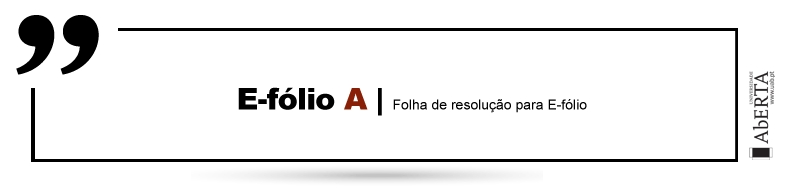
\includegraphics[width=\textwidth]{e-folio-a.jpg}
%
\includegraphics[width=\textwidth]{e-folio-b.jpg}
%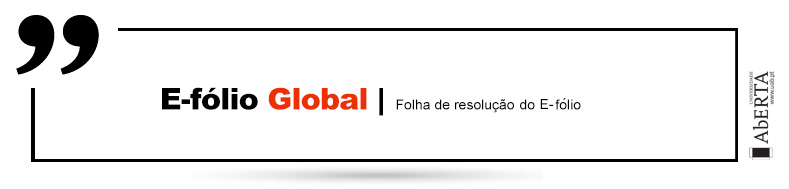
\includegraphics[width=\textwidth]{e-folio-global.jpg}

\paragraph{\textbf{UNIDADE CURRICULAR:}} \UC

\paragraph{\textbf{CÓDIGO:}} \codigoUC

\paragraph{\textbf{DOCENTE:}} \docentes

\paragraph{\textbf{NOME:}} \theauthor

\paragraph{\textbf{N.º DE ESTUDANTE:}} \numeroEstudante

\paragraph{\textbf{CURSO:}} \curso

\paragraph{\textbf{DATA DE ENTREGA:}} \thedate


\section{}

\subsection{}

\begin{theorem}[Somatório de números naturais]
	Para $n \in \mathbb{N}$, tem-se que $\sum_{k = 1}^n k = \frac{n(n+1)}{2}$.
\end{theorem}

\begin{proof}
	\; \\
	Caso base $n = 1$, tem-se que 1 = 1, pelo que verifica o caso base.\\
	Fixado $n \in \mathbb{N}$, vamos supor:
	\begin{align*}
		\sum_{k = 1}^n k &= \frac{n(n+1)}{2} &&\text{(Hipótese de Indução)}
		\intertext{Pretende-se provar:}
		\sum_{k = 1}^{n + 1} k &= \frac{(n + 1)(n+2)}{2} &&\text{(Tese de Indução)}
		\intertext{Passo de Indução:}
		\sum_{k = 1}^{n + 1} k &= n + 1 + \sum_{k = 1}^n k
		\overset{\text{\tiny passo de indução}}{=}
		n + 1 + \frac{n (n + 1)}{2} \\
							   &= \frac{n (n + 1) + 2(n + 1)}{2}
							   = \frac{(n +2)(n + 1)}{2}
	\end{align*}
	\\
\end{proof}


\nocite{uabefoliotemplate}
\printbibliography[heading=bibintoc,title={Bibliografia}]
\listoftheorems[title={Lista de Teoremas}]

\end{document}
